\subsection{Phân tích phương sai một nhân tố (Single-factor ANOVA)}

Dữ liệu:
\begin{itemize}
    \item Y: là một biến phụ thuộc (có tính liên tục).
    \item X: là một biến nhân tố hay biến giải thích (có tính phân loại).
\end{itemize}
Mục tiêu:
\begin{itemize}
    \item Đánh giá xem biến nhân tố X có ảnh hưởng đến biến phụ thuộc Y hay không?
    \item Nói cách khác:
    \[
        H_{0}: \mu_{1} = \mu_{2} = \mu_{3} = \dots = \mu_{n}
        \]
        \[
        H_{1}: \exists i, j \text{ sao cho } \mu_{i} \neq \mu_{j}
        \]
\end{itemize}
%mùa ảnh hưởng tới phí giao hàng
Chúng em quyết định sẽ kiểm định xem, việc các mùa (season) sẽ ảnh hưởng như thế nào đến phí giao hàng (delivery\_charges) bằng phương pháp phân tích phương sai ANOVA một nhân tố. Dưới đây là phân tích phương sai ANOVA một nhân tố cho mẫu thống kê ( hàm phân tích đã được tích hợp sẵn trong R) :

\begin{figure}[!htbp]
    \centering
    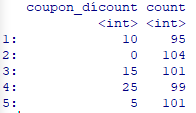
\includegraphics[width=0.4\linewidth]{graphics/5.3.1.png}
    \caption{Phân tích phương sai ANOVA xét sự ảnh hưởng của mùa (season) đến phí giao hàng(delivery\_charges)}
\end{figure}

Xem hình trên ta thấy kết quả, giá trị p-value (tức Pr(>F)) là rất nhỏ hơn ngưỡng ý nghĩa phổ biến (0.05). Do đó, có đủ bằng chứng thống kê rất mạnh để kết luận rằng, các mùa (season) có ảnh hưởng rất mạng đến phí giao hàng (delivery\_charges). Nói cách khác, sự khác biệt về phí giao hàng giữa các mùa không có yếu tố ngẫu nhiên.

%yêu cầu giao hàng nhanh ảnh hưởng tới phí giao hàng

Chúng em quyết định sẽ kiểm định xem, việc khách hàng yêu cầu giao hàng nhanh (is\_expedited\_delivery) sẽ ảnh hưởng như thế nào đến phí giao hàng (delivery\_charges) bằng phương pháp phân tích phương sai ANOVA một nhân tố. Dưới đây là phân tích phương sai ANOVA một nhân tố cho mẫu thống kê ( hàm phân tích đã được tích hợp sẵn trong R) :
\begin{figure}[!htbp]
    \centering
    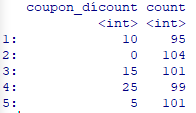
\includegraphics[width=0.4\linewidth]{graphics/5.3.1.png}
    \caption{Phân tích phương sai ANOVA xét sự ảnh hưởng của mùa (season) đến phí giao hàng(delivery\_charges)}
\end{figure}
